\documentclass[border=0.5mm,11pt]{standalone}

% !TeX program = lualatex

\usepackage{../pacchetti-immagini}


\definecolor{turquoise}{RGB}{0, 247, 230}
\definecolor{goldenyellow}{RGB}{255, 218, 66}
\definecolor{fuchsia}{RGB}{255, 0, 172}

%%%%%%%%%%%%%%%%%%%%%%%%%%%%%%%%%%%%%%% HEAD COMMANDS	
\newtheorem{theorem}{Theorem}[section]

\newtheorem{corollary}[theorem]{Corollary}

\newtheorem{lemma}[theorem]{Lemma}

\newtheorem{prop}[theorem]{Proposition}

\theoremstyle{definition}
\newtheorem{definition}{Definition}[section]

\theoremstyle{remark}
\newtheorem*{remark}{Remark}

\newcommand{\EAK}[1]{\textcolor{red}{EAK: #1}}
\newcommand{\VS}[1]{\textcolor{cyan}{VS: #1}}

%%%%%%%%%%%%%%%%%%%%%%%%%%%%%%%%%%%%%%% MATH SYMBOLS
\newcommand{\R}{{\mathbb{R}}}
\newcommand{\N}{{\mathbb{N}}}

 \newcommand{\pprec}{\prec\mathrel{\mkern-5mu}\prec}






\begin{document}
\begin{tikzpicture}[]
\draw[turquoise, ultra thick, ->] (0,0) -- (0,14);

\filldraw[black] (0,1) circle (1pt);
\draw[black] (0,1) -- (3,0) node[inner sep=0pt]
{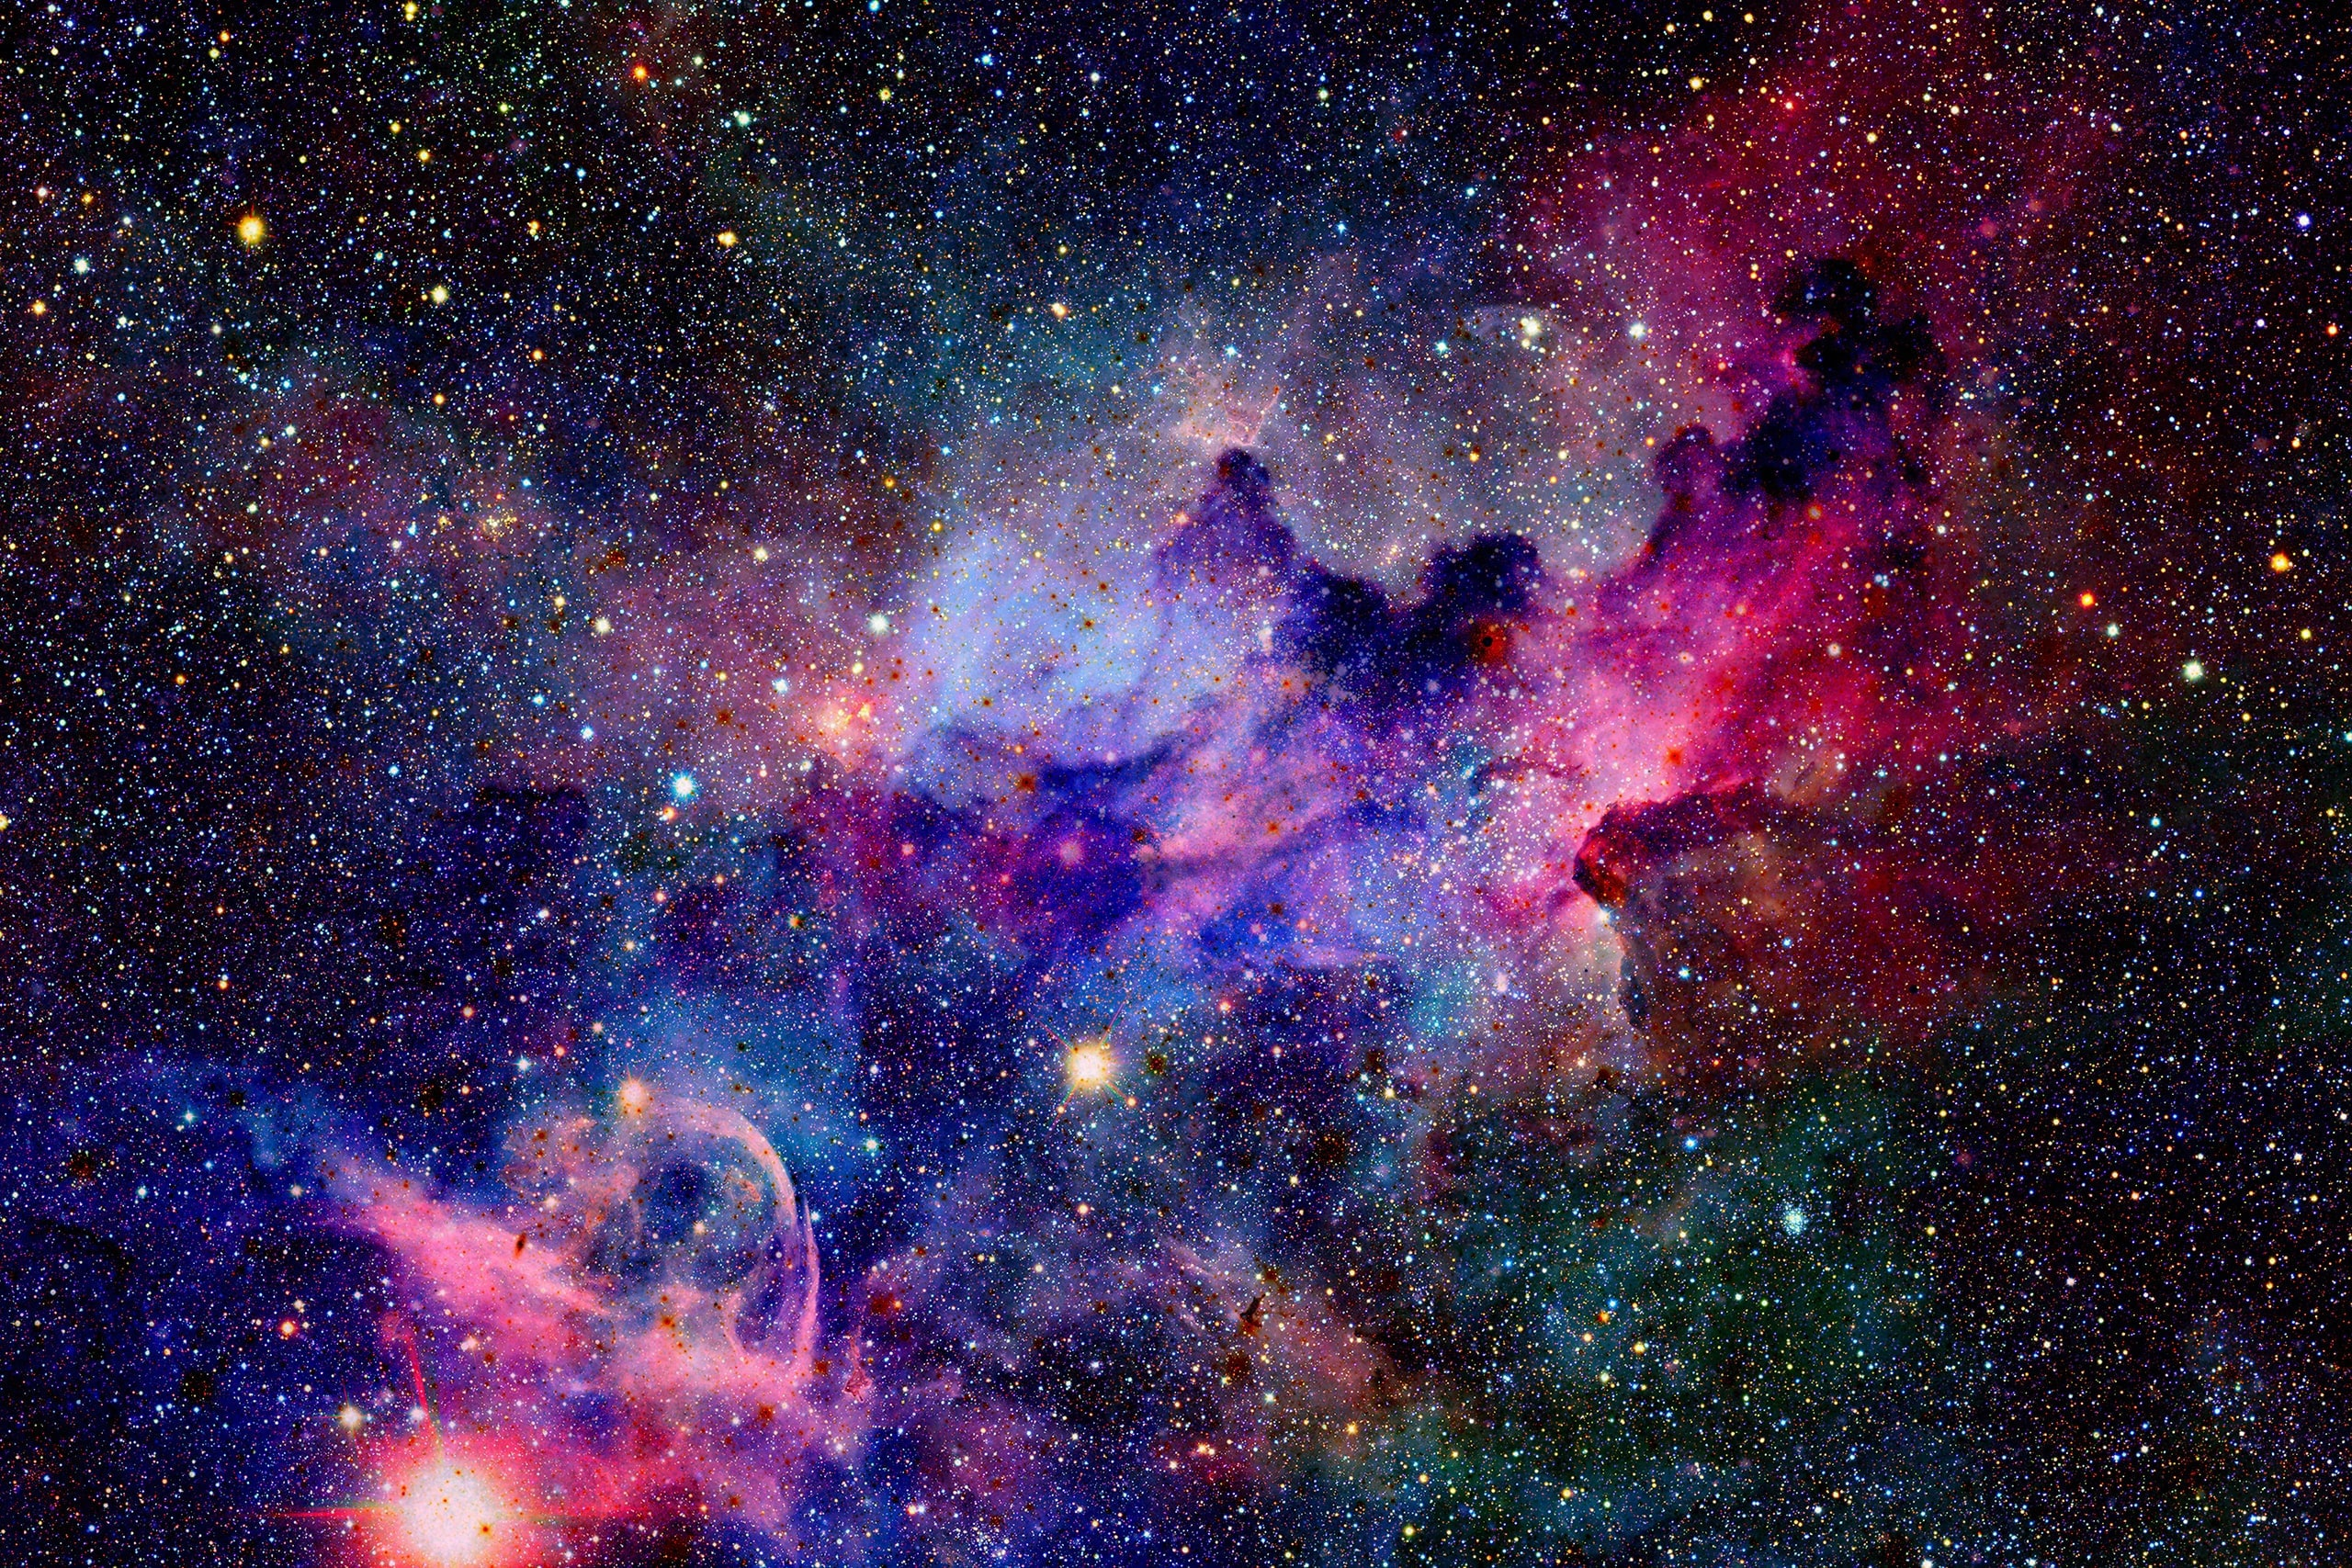
\includegraphics[width=.2\textwidth]{nebula-02.jpg}};
\node at (0.88,0) {\emph{Nebula}};
\begin{scope}[xshift=5cm, yshift=-0.5cm]
    \draw[gray, thick] (0,0) -- (3, 0) -- (5,1) -- (2,1) --cycle;
    \foreach \i in {1,2}{
        \draw[gray] (\i, 0) -- (\i+2, 1);
        \draw[gray] (2*\i/3, \i/3) -- (3 + 2*\i/3, \i/3);
    }
    \node at (0.3, 0.7) {\emph{Flat}};
\end{scope}

\filldraw[black] (0,3) circle (1pt);
\draw[black] (0,3) -- (3,3) node[inner sep=0pt]
{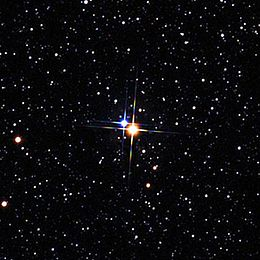
\includegraphics[width=.2\textwidth]{Albireo2.jpg}};
\node at (0.88,2.5) {\emph{Star}};
\node at (8,2.8) {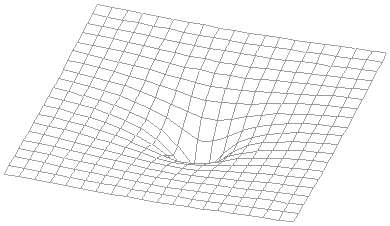
\includegraphics[width=.37\textwidth]{weak-curved.png}};
\node[label={[align=left]\emph{Weakly}\\\emph{Curved}}] at (5.4,3) {};

\draw[goldenyellow, ultra thick, ->] (3, 7) -- (3, 10.5);
\draw[goldenyellow, ultra thick, ->] (3.2, 7) to[out=90, in=-140] (4.5, 10);
\draw[goldenyellow, ultra thick, ->] (3.4, 7) to[out=90, in=-170] (6, 9);
\node[label={[align=left]\emph{Hawking}\\\emph{Radiation}}] at (7.8,8.2) {};

\filldraw[black] (0,5) circle (1pt);
\draw[black] (0,5) -- (3,6) node[inner sep=0pt]
{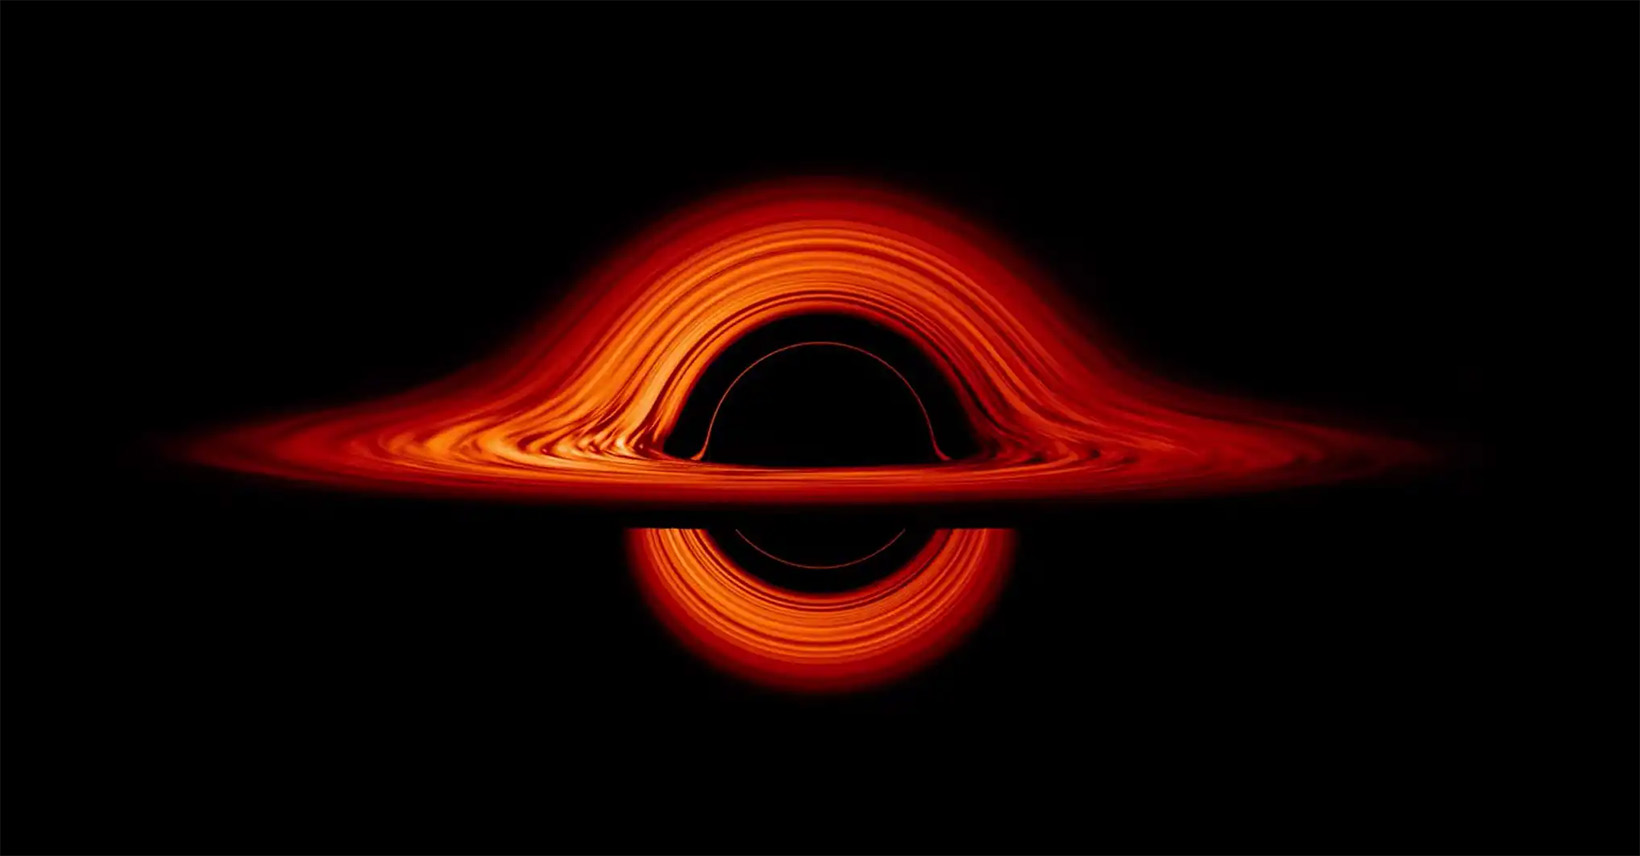
\includegraphics[width=.2\textwidth]{bh.jpg}};
\node[label={[align=left]\emph{Black}\\\emph{Hole}}] at (0.88,5.5) {};
\node at (7.5,6) {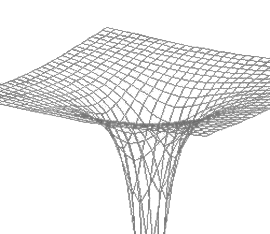
\includegraphics[width=.3\textwidth]{strongly-curved.png}};
\node[label={[align=left]\emph{Strongly}\\\emph{Curved}}] at (5.4,5) {};

\filldraw[black] (0,12) circle (1pt);
\draw[black] (0,12) -- (3,12);
\filldraw (1.7,11) rectangle (4, 13.3);
\node[label={[align=left]\emph{Empty}\\\emph{Space}}] at (0.88,10.7) {};
\begin{scope}[xshift=5cm, yshift=11cm]
    \draw[gray, thick] (0,0) -- (3, 0) -- (5,1) -- (2,1) --cycle;
    \foreach \i in {1,2}{
        \draw[gray] (\i, 0) -- (\i+2, 1);
        \draw[gray] (2*\i/3, \i/3) -- (3 + 2*\i/3, \i/3);
    }
    \node at (0.3, 0.7) {\emph{Flat}};
\end{scope}

\node[mexican, minimum size = 0.5cm, mirrored, female] (A) at (9,10.5){Alice};

\node[cowboy, minimum size = 0.5cm, mirrored] (A) at (9.5,1.2){Bob};

\end{tikzpicture}
\end{document} 


	
	
	
	
	



